% This is "sig-alternate.tex" V2.0 May 2012
% This file should be compiled with V2.5 of "sig-alternate.cls" May 2012
%
% This example file demonstrates the use of the 'sig-alternate.cls'
% V2.5 LaTeX2e document class file. It is for those submitting
% articles to ACM Conference Proceedings WHO DO NOT WISH TO
% STRICTLY ADHERE TO THE SIGS (PUBS-BOARD-ENDORSED) STYLE.
% The 'sig-alternate.cls' file will produce a similar-looking,
% albeit, 'tighter' paper resulting in, invariably, fewer pages.
%
% ----------------------------------------------------------------------------------------------------------------
% This .tex file (and associated .cls V2.5) produces:
%       1) The Permission Statement
%       2) The Conference (location) Info information
%       3) The Copyright Line with ACM data
%       4) NO page numbers
%
% as against the acm_proc_article-sp.cls file which
% DOES NOT produce 1) thru' 3) above.
%
% Using 'sig-alternate.cls' you have control, however, from within
% the source .tex file, over both the CopyrightYear
% (defaulted to 200X) and the ACM Copyright Data
% (defaulted to X-XXXXX-XX-X/XX/XX).
% e.g.
% \CopyrightYear{2007} will cause 2007 to appear in the copyright line.
% \crdata{0-12345-67-8/90/12} will cause 0-12345-67-8/90/12 to appear in the copyright line.
%
% ---------------------------------------------------------------------------------------------------------------
% This .tex source is an example which *does* use
% the .bib file (from which the .bbl file % is produced).
% REMEMBER HOWEVER: After having produced the .bbl file,
% and prior to final submission, you *NEED* to 'insert'
% your .bbl file into your source .tex file so as to provide
% ONE 'self-contained' source file.
%
% ================= IF YOU HAVE QUESTIONS =======================
% Questions regarding the SIGS styles, SIGS policies and
% procedures, Conferences etc. should be sent to
% Adrienne Griscti (griscti@acm.org)
%
% Technical questions _only_ to
% Gerald Murray (murray@hq.acm.org)
% ===============================================================
%
% For tracking purposes - this is V2.0 - May 2012

\documentclass{sig-alternate}

\usepackage{caption}
\usepackage{subcaption}
\usepackage{graphicx}
\usepackage{xcolor}
\newcommand\todo[1]{\textcolor{red}{#1}}


\begin{document}
%
% --- Author Metadata here ---
\conferenceinfo{SIGIR}{'14 Gold Coast, Australia}
%\CopyrightYear{2007} % Allows default copyright year (20XX) to be over-ridden - IF NEED BE.
%\crdata{0-12345-67-8/90/01}  % Allows default copyright data (0-89791-88-6/97/05) to be over-ridden - IF NEED BE.
% --- End of Author Metadata ---

\title{On a Tip of Your Search: Evaluating Effect of Strategic Search Tips on User Success in Complex Informational Search Tasks}

%
% You need the command \numberofauthors to handle the 'placement
% and alignment' of the authors beneath the title.
%
% For aesthetic reasons, we recommend 'three authors at a time'
% i.e. three 'name/affiliation blocks' be placed beneath the title.
%
% NOTE: You are NOT restricted in how many 'rows' of
% "name/affiliations" may appear. We just ask that you restrict
% the number of 'columns' to three.
%
% Because of the available 'opening page real-estate'
% we ask you to refrain from putting more than six authors
% (two rows with three columns) beneath the article title.
% More than six makes the first-page appear very cluttered indeed.
%
% Use the \alignauthor commands to handle the names
% and affiliations for an 'aesthetic maximum' of six authors.
% Add names, affiliations, addresses for
% the seventh etc. author(s) as the argument for the
% \additionalauthors command.
% These 'additional authors' will be output/set for you
% without further effort on your part as the last section in
% the body of your article BEFORE References or any Appendices.

\numberofauthors{2} 

\author{
% 1st. author
\alignauthor
Denis Savenkov\\
       \affaddr{Emory University}\\
       \email{dsavenk@emory.edu}
% 2nd. author
\alignauthor
Eugene Agichtein\\
       \affaddr{Emory University}\\
       \email{eugene@mathcs.emory.edu}
}
\date{17 February 2014}
% Just remember to make sure that the TOTAL number of authors
% is the number that will appear on the first page PLUS the
% number that will appear in the \additionalauthors section.

\maketitle
\begin{abstract}
Search engine is a ubiquitous tool used by millions of people on a daily basis.
However, it is usually the case, that certain skills are required in order to use it efficiently.
Modern search engines provide users with some automatic assistance during their searches and arguably one of the most successful technique is query suggestion.
Although it is very effective for relatively popular topics, there are still many tasks that search engines do not handle perfectly and users do not get any assistance and become frustrated \cite{Feild:2010:PSF:1835449.1835458}.
A number of researches has been made to study different ways of user assistance (\cite{Kelly:2009:CQT:1571941.1572006}, \cite{Moraveji:2011:MIU:2009916.2009966}, \cite{marchionini2006toward}).
Displaying search tips is another alternative for automatic user assistance. Previous researches (\cite{Moraveji:2011:MIU:2009916.2009966}) studied the effect of tips, which suggest users some features of search engines that might be optimal for specific search tasks.
However, as the majority of cases when users require assistance (\cite{xie2009understanding}) come from query formulation and refinement stages, the tips studied in \cite{Moraveji:2011:MIU:2009916.2009966} might not be that effective in general.
In this work we study the effect of displaying strategic search tips, which suggest a way of solving a difficult search problem by splitting it into pieces and searching for parts of the question and combining these answers together.
We focus on 2 types of tips: task-specific tips, tailored to a problem user is currently solving and generic tips, describing the general strategy of splitting problem into pieces. 
In the user study conducted using a web search game users were able to follow optimally designed task-specific tips and achieve higher success rate than users who didn't get such assistance.
However, generic tips were shown to be rather distracting and detrimental.
\end{abstract}

% A category with the (minimum) three required fields
\category{H.3.3}{Information storage and retrieval}{Information Search and Retrieval}[query formulation, search process]
%A category including the fourth, optional field follows...

\terms{Measurement, Design, Experimentation, Human Factors}

\keywords{User studies, search interface, experimental design, query reformulation, tactics, tips, suggestions, assistance, efficiency.}

\section{Introduction}
Solving a search problem involves 2 parties: a system that answers queries and a user who interacts with the system. Asking the right questions and interacting with the system in a right way is as important (or even more important) than the quality of system answers \todo{[can we support this with some citation]}. The importance of user interactions is even more important for difficult queries which are still not answered correctly by the modern search engines \todo{[cite robustness paper]}. 

The importance of helping users to interact with the system is well understood and various researches studies different ways of user assistance \todo{[a list of citations goes here]}. But unfortunately, modern search engines are still limited in providing user feedback and suggestions. It is a standard to offer query syntax correction to help fixing typos and misspellings, query suggestions to guide users to ``better'' queries, rich search results representations to help users choose which results to click on or to give an answer \todo{Is there something else?}.

However, these tools are limited in assisting users to solve difficult informational search task. The ability to formulate good search queries and use search tools as efficiently as possible becomes the crucial factor towards the overall success. People have different skills and abilities and the effect of these variables to successful search is sometimes more important than retrieval performance \todo{[need to support this with something]}. 

\todo{[Need some transition to why we study these particular type of tips for these particular type of search problems. Possibly link to agoogleaday as example of difficult search problems]}. 

In this paper we study the effect of strategic search hints, designed to guide user in splitting the original problem into pieces and combining results for subproblems together. More specifically we manually designed 2 type of tips: task-specific, which present a way of correctly solving the questions and generic, which explains ``divide and conquer'' strategy, i.e. splitting the original question into pieces and combining answers to these pieces together. The user study was conducted in a form of a search game and it reveiled that users were able to follow carefully designed task-specific hints and this lead to increase in success rate. However, generic tips were probably distracting to the user and the success rate dropped as compared to not seeing any search tips.
This suggests that \todo{[what?]}.

\section{Related Work}

% Helping users to develop their search skills was included as one of the key research directions by \cite{Allan:2012:FCO:2215676.2215678}.


There has been considerable amount of work on search assistance and improving user experience with feedback, suggestions and hints. Interactive information retrieval and human-computer information retrieval \cite{marchionini2006toward} focuses on interactions between users and search systems. Graphical techniques can be used to visually represent large-scale collections of information and help searchers in their tasks \cite{card1999readings}.

Results of the study in \cite{xie2009understanding}, which focused on identification of different categories of help-seeking situations, demonstrates that in 41.5\% of the cases users were seeking for help to refine their searches followed by inability to construct search statements in 18\% of the cases. 
Individual terms (\cite{ruthven2003survey}) and queries suggestion (\cite{Jones:2006:GQS:1135777.1135835},\cite{Bhatia:2011:QSA:2009916.2010023},\cite{Cao:2008:CQS:1401890.1401995}) are among the most popular techniques for helping users to augment their queries.
The study from \cite{Kelly:2009:CQT:1571941.1572006} demonstrated that users prefer query suggestions over term relevance feedback and that good manually designed suggestions improve retrieval performance.
Query suggestion methods usually provide previous queries that are similar to the query of interest and work better for popular information needs \cite{Bhatia:2011:QSA:2009916.2010023}.

When query or term suggestions are not efficient, it is still possible to help users by providing potentially useful search hints. An adaptive tool providing tactical search suggestions was presented in \cite{Kriewel2007} and users reported overall satisfaction with its automatic non-intrusive advices. Modern search engines have many features that are not typically used by a average user, but can be very useful in particular situations as shown in \cite{Moraveji:2011:MIU:2009916.2009966}. The study demonstrated the potential effectiveness of tactical search feature tips and their teaching effect.

The major differences of this work from \cite{Moraveji:2011:MIU:2009916.2009966} is the type of search tips used.
Rather than suggesting users the available search features to use, this work focuses on strategic search tips, designed to help users solve difficult informational questions.
Many informational questions cannot be answered by a single web query and require splitting the task into pieces and combining partial answers into new searches. From our studies we noticed that users do not actively use this tactic and usually keep trying to reformulate their query expecting to find the query that will give them the correct result.
However, in these tasks it is hard to come up with a good hint which will help all the users.
In this study we are evaluating the effect that task-specific manually designed strategic tips as well as generic task-independent tips might have on user experience and success rate.

% Not relevant
% The effect of different factors on users' perception of search task difficulty was studied in \cite{liu2011understanding}. The results demonstrated that users' prior expectations of task difficulty is likely to be inaccurate and perceived difficulty change before and after users worked on the task is affected by task types.

% Good, but don't know where to put this.
% Search skills can be trained \cite{Moraveji:2011:MIU:2009916.2009966}. For example, Google offers courses\footnote{http://www.powersearchingwithgoogle.com} designed to improve ones efficiency in solving difficult search tasks and interacting with a modern search engine.

\section{Tips for Difficult Search Tasks}
To estimate the effect of search tips on user behavior and success we conducted a user study using Amazon Mechanical Turk platform\footnote{http://www.mturk.com/}. 
The motivation to find the correct answer is very important for the study, thus we decided to pose the task as a web search game similar to a Google a Day\footnote{http://www.agoogleaday.com/} and uFindIt \cite{Ageev:2011:FYG:2009916.2009965}. 

\subsection{Web Search Game}

\begin{figure}
\centering
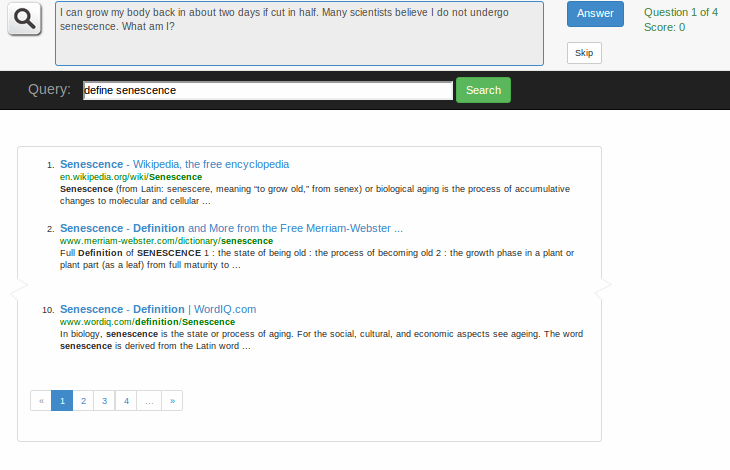
\includegraphics[scale=0.29]{img/ufindit}
\caption{The interface of the search game used in the study}
\label{figure:ufindit}
\end{figure}


The web search game used for the study asks users to find answers to several questions using the provided web search interface. Figure \ref{figure:ufindit} shows the interface of the game. 
% Rules
At the beginning of the game users are instructed to use only the search interface provided.
Answers should actually be found using web search.
In a rare occurrence that a user might know the answer to a question she is instructed to ignore the prior knowledge and use the search anyway.
Since tasks might be too difficult a chance to skip a question was provided, although users were instructed that effort put into solving a question will be evaluated.

In the previous experiments we've noticed that with difficult search tasks Mechanical Turk workers tend to skip the validation phase \cite{Ageev:2011:FYG:2009916.2009965} and submit the first possible answer found when even shallow analysis reveals that it is incorrect.
To overcome this problem the submitted answers were automatically checked for correctness (a presence of the required keyword).
If the answer was incorrect a dialog popped up and a player could continue search.

% Technology
The game search interface was based on API of one of the major web search engines. All search results were cached so that users asking the same query get the same results. Moreover, all links to web pages were rewritten to use our caching HTTP proxy.

% Finally
At the end of the game a questionnaire was presented asking for feedback on user satisfaction with the game, prior experience and other comments.

\subsection{Search Tasks Description}

The tasks for the study were borrowed from the a Google a Day questions archive. Unfortunately, a lot of web pages discussing solutions to these questions exist. So we had to filter search results and exclude all pages that mention a major part of the search question or ``a google a day'' phrase.
To keep users focused throughout the whole game we decided to limit the number of questions to 4.
Table \ref{table:tasks} describes all 4 tasks.

\begin{table*}
\centering
\caption{Search tasks used for the study}
\label{table:tasks}
\begin{tabular}{|l|p{6cm}|p{8cm}|} \hline
Task ID & Task Text & Answer \\ \hline
Task 1 (``hydra'') & I can grow my body back in about two days if cut in half. Many scientists believe I do not undergo senescence. What am I? & Senescence means ``biological aging''. Hydra is considered biologically immortal and regenerates fast. \\ \hline
Task 2 (``quirinus'') & Of the Romans "group of three" gods in the Archaic Triad, which one did not have a Greek counterpart? & Archaic Triad includes Jupiter, Mars and Quirinus. Among those Quirinus didn't have a Greek counterpart.\\ \hline
Task 3 (``dinosaur'') & As George surveyed the ``waterless place'', he unearthed some very important eggs of what animal? & Waterless place is the translation of the Mongolian word "Gobi" or ``Gobi Desert''. George Olsen found the first whole dinosaur eggs in 1923. \\ \hline
Task 4 (``cherokee'') & If you were in the basin of the Somme River at summers end in 1918, what language would you have had to speak to understand coded British communications? & Cherokee served as code talkers in the Second Battle of the Somme. \\ \hline
\end{tabular}
\end{table*}

\subsection{Search Tips}
The tasks used for the game are examples of complex informational search problems and usually require several searches. Questions have multiple parts and to solve them it is helpful to search for answers to parts of the questions and then combine them.

We studies 2 types of search tips: task specific and generic. Task specific hints were constructed from one of the possible solutions to the question and described one way to search and find the answer. Generic hint described the general strategy that can be applied to many difficult informational search task.
The actual tips shown to the players are described below.

Generic hint was the same for all tasks and looked the following way:
\vspace{-1mm}
\begin{enumerate} \itemsep0pt \parskip0pt \parsep0pt
\item Split question into 2 or more logical parts
\item Find answers to the parts of the question
\item Use answers to the parts of the question to find answer to the full question
\end{enumerate}
\vspace{-1mm}
For example:\\
Question: The second wife of King Henry VIII is said to haunt the grounds where she was executed. What does she supposedly have tucked under her arm?
\vspace{-1mm}
\begin{enumerate} \itemsep0pt \parskip0pt \parsep0pt
\item Search [second wife King Henry VIII] to find Anne Boleyn.
\item Search [Anne Boleyn under arm] to find that her ghost is in the London Tower where she is said to carry her head tucked underneath her arm.
\end{enumerate}

Specific hints were designed for each question separately and presented a way to solve the problem by searching for a specific parts of the question.
Specific tip for Task 1:
\vspace{-1mm}
\begin{enumerate} \itemsep0pt \parskip0pt \parsep0pt
\item Find what is senescence
\item Find who do not undergo senescence
\item Find animals who can regenerate body and choose the one that satisfy both conditions
\end{enumerate}
\vspace{-1mm}
Tip for Task 2:
\vspace{-1mm}
\begin{enumerate} \itemsep0pt \parskip0pt \parsep0pt
\item Find the names of the gods from the Archaic triad
\item For each of the gods find a Greek counterpart
\end{enumerate}
\vspace{-1mm}
Tip for Task 3:
\vspace{-1mm}
\begin{enumerate} \itemsep0pt \parskip0pt \parsep0pt
\item Find what is the ``waterless place'' mentioned in the question?
\item Search for important eggs discovery in this ``waterless place''
\end{enumerate}

To avoid the learning effect demonstrated in \cite{Moraveji:2011:MIU:2009916.2009966} we split users into 3 groups: users who were shown no tips; users who were shown task-specific tips and users who were shown generic tip for all tasks.


\section{Results}
From 199 participants, who accepted the HIT on Amazon Mechanical Turk\footnote{http://mturk.com/}, only 169 moved further than the rules of the game and got to the first questions.
The search tasks were difficult and some players decided to quit the game, thus only 90 players finished the game, from those there were 9 submissions which we filtered out from the future analysis.
The only 2 reasons for that were: lack of effort, e.g. some players skipped several tasks after only a single query; some other submissions indicated usage of external resources such as outside of the game search engine, e.g. the only query asked was the correct answer to the task.
From 81 submissions 10 players indicated in the survey that they didn't see the tips which were shown to them, so we further filtered those submissions and finally we had 71 completed games, which split into the groups of 29, 20, 22 for players who didn't have tips, who had task-specific hints and who had generic tips correspondingly.
\todo{What is missing?}

\subsection{Analysis}

The main characteristic of interest was the search success rate, measured in the number of questions answered correctly by users in different groups. Figure \ref{figure:task_success} plots the fraction of correct answers for players from different groups. As we can see, success rate tend to be higher for users who saw task-specific hint compared to users who didn't see any hint. Somewhat surprising is the fact, that users who saw generic tip were slightly less successful. The difference is more significant in more difficult tasks 1 and 4. This can probably be explained by the fact that generic tip was more difficult to implement and unsuccessful attempts lead to frustration \todo{Sound reasonable?}.

\begin{figure}[ht]
\centering
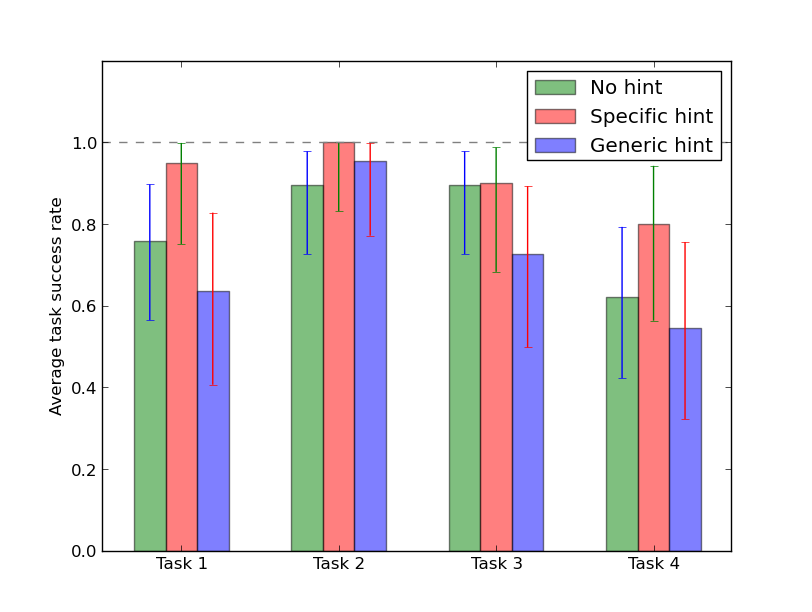
\includegraphics[scale=0.4]{img/success_per_task}
\caption{Success rate per task for each group of participants}
\label{figure:task_success}
\end{figure}

Similar to \cite{Moraveji:2011:MIU:2009916.2009966} we looked at the average time to answer the question (we removed games where a user didn't find the answer and skipped the task), the plot is provided on Figure \ref{figure:task_time}. Here we don't see a clear pattern, for task 1 participants who saw task-specific tip were able to find the answer faster, however this is not the case for task 4. A possible explanation is that the provided tips were not the optimal ones and the problem allowed a faster solution, which was found by users who didn't see the tips \todo{Can I find an example of a search trail?]}. It is worth noting, that users from the generic search tip group had slightly higher variance in success time, which is probably explained by the fact that some users were successful in finding the right way to follow the tip and some other users struggled with it more \todo{Reasonable?}.

\begin{figure}[ht]
\centering
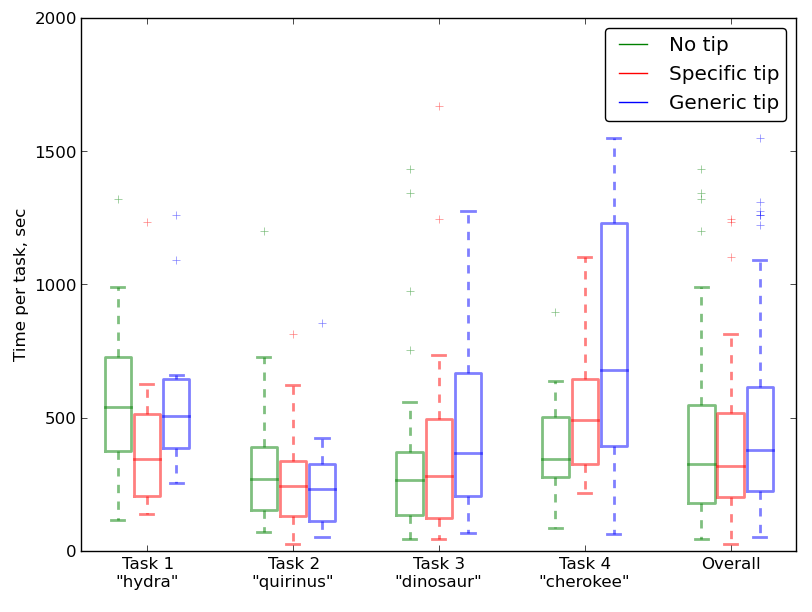
\includegraphics[scale=0.4]{img/time_per_task}
\caption{Task completion time for each group of players}
\label{figure:task_time}
\end{figure}

Another interesting insight comes from the number of incorrect attempts users made. Figure \ref{figure:incorrect} demonstrates the average number of incorrect submissions for all groups of users. Although the variance is high, but there is a tendency, that users who saw task-specific tips made less submission attempts and users who saw generic tip were incorrect slightly more often than users who didn't get any tips during the game. 
This is not in direct correspondence with time spent on the game. The effect can probably be explained by the difference in frustration in each of the user groups. Users who saw a clear strategy to solve the question were less likely to notice plausible, but incorrect solution.
Moreover, by analyzing texts of incorrect answers we can conclude that users sometimes tried to guess the correct answer by typing everything that came in mind.

\begin{figure}[ht]
\centering
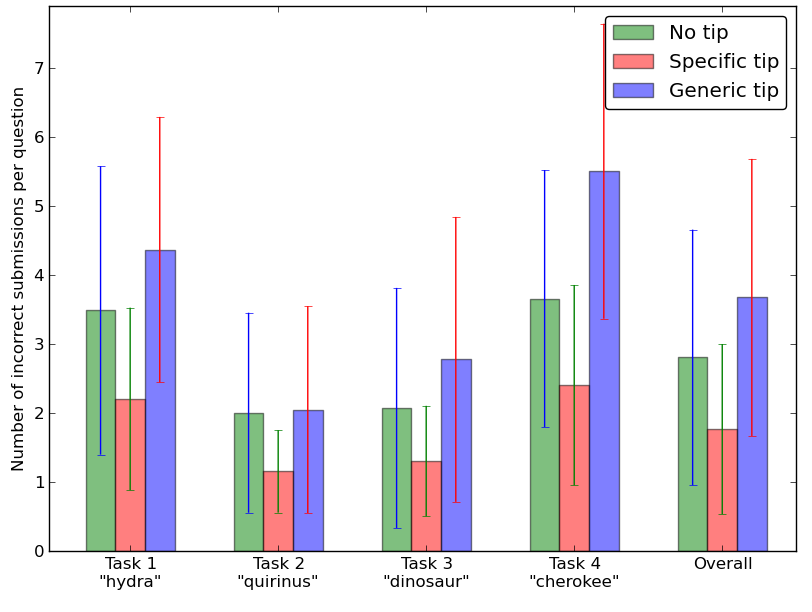
\includegraphics[scale=0.4]{img/incorrect}
\caption{The number of incorrect submission attempts per question for all groups of users}
\label{figure:incorrect}
\end{figure}

Finally, we looked at the surveys left by each group of users.
Figure \ref{figure:survey} presents proportions of different answers to three of the questions: ``How did you like the game?'', ``How difficult was the game?'' and ``Were search tips useful to you?''.
Surprisingly, results for the first question were lower for users who saw tips during the game and users who didn't saw tips liked the game more.
It could be explained by the self-achievement effect, that is lower when users get help even if it wasn't helpful. The answers to the question about game difficulty are in agreement with the success rate: users who saw task-specific tips rates game as being easier than participants who struggled more to get the correct answers. The Figure \ref{figure:survey:useful} shows that users actually found our hints useful for their searches and indicated this in the final survey.

\begin{figure*}[ht]
\centering
\begin{subfigure}[t]{0.3\textwidth}
	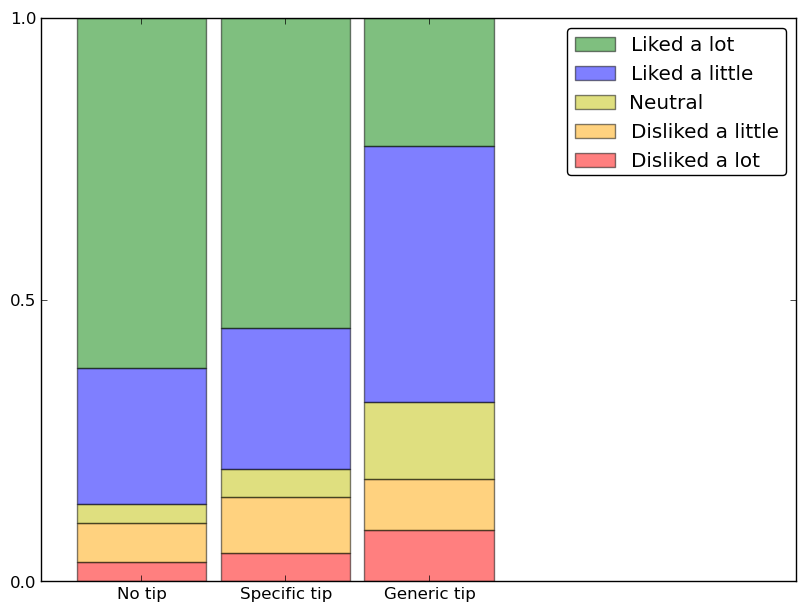
\includegraphics[scale=0.26]{img/liked}
	\caption{How did you like the game?}
    \label{figure:survey:liked}
\end{subfigure}
\begin{subfigure}[t]{0.3\textwidth}
	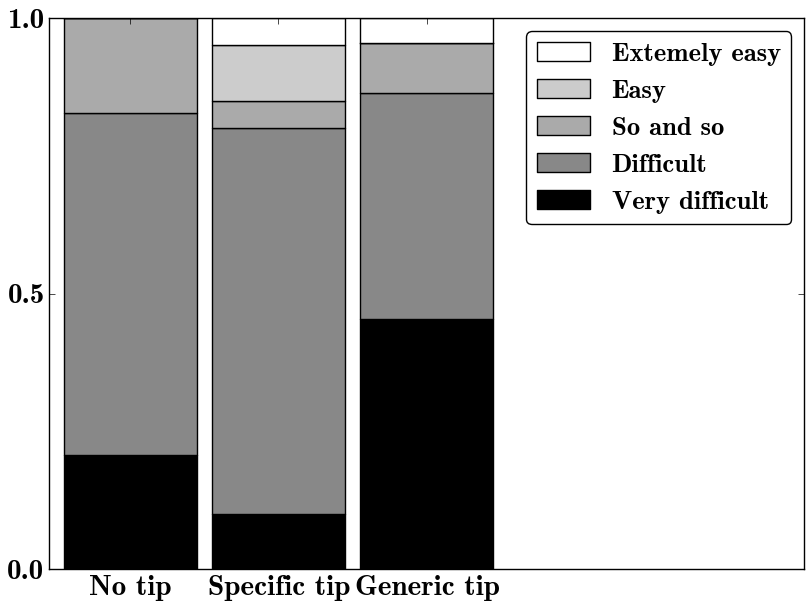
\includegraphics[scale=0.26]{img/difficult}
	\caption{How difficult was the game?}
    \label{figure:survey:difficult}
\end{subfigure}
\begin{subfigure}[t]{0.3\textwidth}
	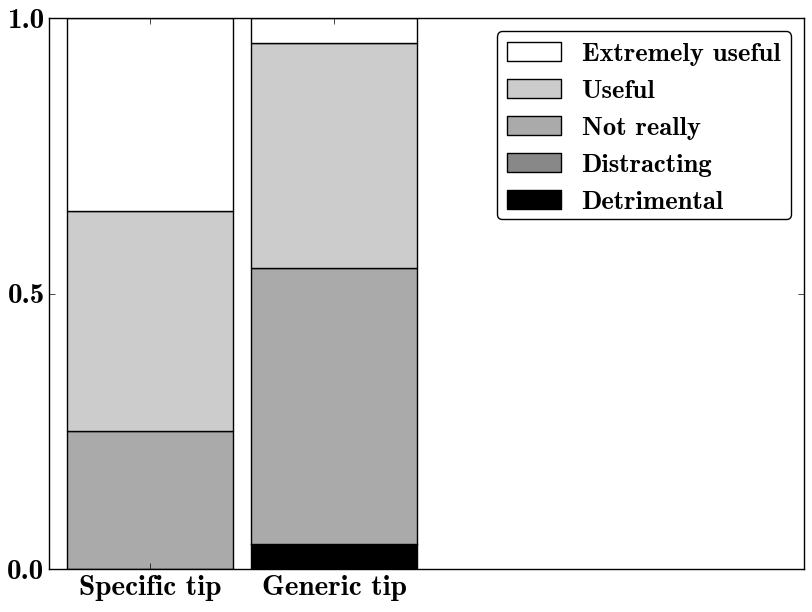
\includegraphics[scale=0.26]{img/useful}
	\caption{Were search tips useful to you?}
    \label{figure:survey:useful}
\end{subfigure}
\caption{Proportions of replies to some of the survey question for each group of users}
\label{figure:survey}
\end{figure*}

\section{Conclusion}
The results of the user study described in this work demonstrated the potential of good strategic search tips and their effect on search success. However, search tips that are too general and hard to implement could be detrimental. Users in our study were less successful when they saw generic strategic search tip. 

% Do I need this in conclusion?
% Surprisingly we noticed that users from groups that were provided with tips during the game liked it slightly less than users who were working by themselves. 


%ACKNOWLEDGMENTS are optional
\section{Acknowledgments}
The authors would like to thank Daniel Russel for providing an archive of questions from ``a Google a Day'' search game.

%
% The following two commands are all you need in the
% initial runs of your .tex file to
% produce the bibliography for the citations in your paper.
\bibliographystyle{abbrv}
\bibliography{sigproc}  % sigproc.bib is the name of the Bibliography in this case
% You must have a proper ".bib" file
%  and remember to run:
% latex bibtex latex latex
% to resolve all references
%
% ACM needs 'a single self-contained file'!
%
%APPENDICES are optional
%\balancecolumns

\end{document}
